\documentclass{report}
\usepackage{graphicx}
\usepackage{float}
\graphicspath{{./images/}} 
\begin{document}
\begin{titlepage}
\begin{center}

{\Huge \bfseries
Stock Market Price Prediction Using Time Series Analysis\\
}~\\%[1cm]

% The '~' is needed because \\ only works if a paragraph has started.

{\large
\emph{A Minor Project Report Submitted
in Partial Fulfillment of Requirements
for the Degree of}\\
}~\\

{ \bfseries
Bachelor of Technology in Information Technology
}\\ [1.3 cm]

{\large
by\\
\begin{longtable}

Nishanta Sarma     & (Roll No. BT/IT/14-28)\\
Dakamanbha Ryngkhlem    & (Roll No. BT/IT/14-13)\\
Devilata Pegu     & (Roll No. BT/IT/14-14)\\

\end{longtable}
}~\\[1cm]

{ \centering
Under the Supervision of \\
\bfseries
Dr. Bubu Bhuyan\\
Associate Professor\\
Department of Information Technology\\
North Eastern Hill University.


}

\vfill


\includegraphics[width=4cm]{nehulogo.jpg}~\\[1cm]

{\large \bfseries
Department of Information Technology\\
School of Technology\\
North-Eastern Hill University, Shillong\\[.5cm]
\small	

December 2017

}

\end{center}
\end{titlepage}


\chapter*{Abstract}
 Stock market price prediction is an ongoing topic where lots of research has been done and is still going on, yet there is still not much succeess. In our project we try to predict the next day stock price using Support Vector Regression Algorithm on data from various sources. We then analyse the result and we get the mean error to be 0.5 approximately.     
\addcontentsline{toc}{chapter}{Abstract}
\chapter*{Acknowledgement}
We are highly thankful to our project guide Dr. Bubu Bhuyan for his valuable time and guidance throughout the course of project which has ultimately lead us towards a fruitful result. His consistent mentoring and inspiration has borne enthusiasm  which made it possible for completion of the project in right time.
\newline
We are grateful to Dr. MD Iftekhar Hussain, Head of the Department of Information Technology, NEHU for providing us with all the facilities available in the department for carrying out this work.
We would like to thank all the faculty and staff members of IT Department for providing us with the required facilities and support for completion of our project.

\vspace{7cm}

\begin{flushright}
Nishanta Sarma (Roll No. BT/IT/14-28)\\
Dakamanbha Ryngkelem (Roll No. BT/IT/14-13)\\
Devilata Pegu (Roll No. BT/IT/14-14)\\
\end{flushright}
\addcontentsline{toc}{chapter}{Acknowledgement}

\chapter*{Declaration}
This is to certify that we have properly cited any material taken from other sources and have obtained permission for any copyrighted material included in this report. We take full responsibility for any code submitted as part of this  project and the contents of this report.\\
% This space is for putting the signatures.
\vspace{7cm}



\begin{flushright}
Nishanta Sarma (Roll No. BT/IT/14-28)\\
Dakamanbha Ryngkhlem (Roll No. BT/IT/14-13)\\
Devilata Pegu (Roll No. BT/IT/14-14)\\
\end{flushright}



\addcontentsline{toc}{chapter}{Declaration}

\begin{center}
\vspace{0.6cm}

\includegraphics[width=4cm]{nehulogo.jpg} \\
\hspace{100mm}Date:

\vspace{10mm}\textsl {To whom it may concern}\\[0.5cm]
\end{center}
\vspace{10mm} This is to certify that  ( Nishanta Sarma(BT/IT/14-28) ,Dakamanbha Ryngkhlem(BT/IT/14-13), 
Devilata Pegu(BT/IT/14-14) ) worked in the project \underline{Stock Market Price Prediction }\newline \underline {Using Time Series Analysis} from 12th July 2017 to 13th November 2017 and has successfully completed the minor  project, in order to partial fulfillment of the requirements for the award of the degree of Bachelor of Technology in Information Technology under my supervision and guidance.


\vfill

\addcontentsline{toc}{chapter}{Certificate from the Supervisor}
\newpage

\begin{center}
\vspace{0.6cm}

\includegraphics[width=4cm]{nehulogo.jpg} \\
\hspace{100mm}Date:


\vspace{10mm}\textsl {To whom it may concern}\\[0.5cm]
\end{center}
 \vspace{10mm} This is to certify that  ( Nishanta Sarma(BT/IT/14-28) ,Dakamanbha Ryngkhlem(BT/IT/14-13), 
Devilata Pegu(BT/IT/14-14) ) worked in the project \underline{Stock Market Price Prediction }\newline \underline {Using Time Series Analysis} from 12th July 2017 to 13th November 2017 and has successfully completed the minor  project, in order to partial fulfillment of the requirements for the award of the degree of Bachelor of Technology in Information Technology under my supervision and guidance.


\vfill

\begin{flushleft}
\newline
\textbf{External Examiner} \hspace{70 mm} \textbf{Head} 
\end{flushleft}

\begin{flushright}
 
Department of Information Technology \\
North-Eastern Hill University \\
Shillong-793022, Meghalaya, India \\
\end{flushright}


\addcontentsline{toc}{chapter}{Certificate from the Head}





\tableofcontents{}

\chapter{Introduction}

 
\section{Aim}

The aim of this project is to approximate the next day closing stock price given the previous days data. We try to do this by collecting data from dispartate sources.
\newpage

\section{Motivation}

According to Efficient market hypothesis, The stock market is totally random but financial firms and companies like Goldmansachs have still been trying to make predictive models about the stock market and there's also investors like Warren Buffet who have become quite successful by their investment policies.\newline

We on the other hand choose this topic because of our interest in the underlying and the most rapidly growing technology The technology namely machine learning and Artificial intelligence which are used in many sectors ranging from bioinformatics, astrophysics computer science, statistics etc.   
\newpage
\section{Platform used}

We choose the python programming language for our project because of the following reasons. \newline
\newline
1.Good readability \newline \newline
2.The open source community of python is very active and has scope for help if we get stuck.\newline \newline
3.Python is one of the top languages used for machine learning and and A.I as the libraries available
in python allows easy programming and the developer can focus more on the machine learning part rather than
focusing on the programming part alone.\newline \newline
The libraries used in our project are as follows- \newline \newline
1.Numpy- It is a library for the Python programming language, adding support for large, multi-dimensional arrays and matrices, along with a large collection of high-level mathematical functions to operate on these arrays.\newline
\newline \newline
2.Pandas- pandas is a Python package providing fast, flexible, and expressive data structures designed to make working with structured (tabular, multidimensional, potentially heterogeneous) and time series data both easy and intuitive. It aims to be the fundamental high-level building block for doing practical, real world data analysis in Python.\newline
\newline \newline
3.Matplotlib-Matplotlib is a Python 2D plotting library which produces publication quality figures in a variety of hardcopy formats and interactive environments across platforms. Matplotlib can be used in Python scripts, the Python and IPython shell, the jupyter notebook, web application servers, and four graphical user interface toolkits.\newline
\newline \newline
4.Scikit-learn- It provides simple and efficient tools for data mining and data analysis, accessible to everybody and
reusable in various contexts. Built on Numpy, Scipy and matplotlib
\newpage
\chapter{Background Study}
\section{Work Done in this field}
Here are some of the ways by which Stock Market prediction has been done so far-

Using Sentiment Analysis-Since stock market is very sensitive to external information, It doesn't merely depends on the 
previous stocks alone. Attempts have been made to predict stock prices by studying public sentiments of stocks.But none of
the publicly available models have been very successful \newline

Using Clustering Techniques- Clustering techniques like Gaussian Mixture Model have been used to try and predict the volatility of the stock market. But the main dificulty in this type of predictive models is to decide on the number of clusters. Very detailed analysis of the market data needs to be done to decide on the number of clusters.\newline

Using Supervised learning algorithms- Learning algorithms like Artificial Neural Networks(ANN), Support Vector Machines,Decision Trees have been used to build models to predict stock moments.

So after going through some of the work done in this field we went with our project by at first understanding the very basics of how machine learning alogrithm works that is to optimize an objective function by minimizing the error.\newline\newline
After studying at a high level that how machine learning algorithm works we looked at a few machine learning papers namely Applications of Machine learning in Stock prediction and the Mininmum correlation paper.\newline\newline
We studied linear regression in detail and then went on to study Support Vector Regression and Regression using Artificial Neural Networks(ANN) in detail as it was mentioned in the first paper then we decided to go with Support Vector Regression because of the followuing reasons.\newline
\newline
1. We can't use linear regression because the stock market is non-linear.
\newline\newline
2. The Backpropagation algorithm which is the core algorithm used in an ANN was given in a paper in 1986 by Geoffrey Hinton 
   but neural networks gained much popularity only from 2007-2008 as neural nets required both lot of data and computing power and both were lacking during the 90's.\newline\newline
 So, since we had  data only for  1 month we decided to go with Support Vector Regression(SVR)

 \newpage 
\section{Description about algorithms Studied}
\subsection{Linear regression}
In statistics, linear regression is a linear approach for modeling the relationship between a scalar dependent variable y and one or more explanatory variables (or independent variables) denoted X. The case of one explanatory variable is called simple linear regression. For more than one explanatory variable, the process is called multiple linear regression.
In this type of regression we try and find the best curve that fit our data by at first deciding on the type of curve that we want to fit.Suppose we want to fit a straight line whose equation is given as $$y(predicted)=mx+b$$
Given a training set for x and y we need to find the best fit by choosing the best parameter m and b. We can do it by minimizing an error function such as the squared error which is a convex function.
 $$Error=\sum_{i=1}^{m} (y(predicted)-y_{i})^2/m$$
 where m is the number of training examples
 We minimize this error function by using an algorithm like gradient descent and concurrently go on updating the values of the parameters m and b till we reach convergence.\newline
 $$m = m - a*\frac{dError}{dm}$$
 $$b = b - a*\frac{dError}{db}$$
 where a is the learning rate
\begin{figure}[H]
 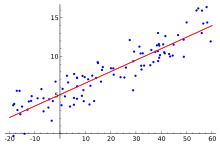
\includegraphics[width=\linewidth]{linear_regression.png}
 \caption{Linear Regression}
\end{figure}


\newpage

\subsection{Support Vector Machine - Regression (SVR)}

Support Vector Machine can also be used as a regression method, maintaining all the main features that characterize the algorithm (maximal margin). The Support Vector Regression (SVR) uses the same principles as the SVM for classification, with only a few minor differences. First of all, because output is a real number it becomes very difficult to predict the information at hand, which has infinite possibilities. In the case of regression, a margin of tolerance (epsilon) is set in approximation to the SVM which would have already requested from the problem. But besides this fact, there is also a more complicated reason, the algorithm is more complicated therefore to be taken in consideration. However, the main idea is always the same: to minimize error, individualizing the hyperplane which maximizes the margin, keeping in mind that part of the error is tolerated.

\begin{figure}[H]
 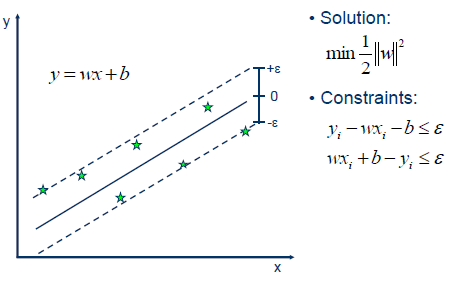
\includegraphics[width=\linewidth]{svr0.png}
 \caption{Basic Regression}
\end{figure}

\begin{figure}[H]
 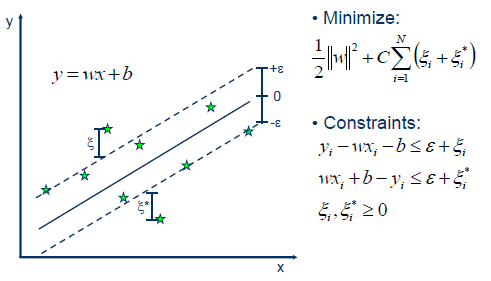
\includegraphics[width=\linewidth]{svr.png}
 \caption{Basic Regression}
\end{figure}
Linear SVR		
$$ y = \sum_{i=1}^{n} (a_{i} - a_{i}^*).<x_{i},x> + b $$
Non-linear SVR		
The kernel functions transform the data into a higher dimensional feature space to make it possible to perform the linear separation.		
$$ y = \sum_{i=1}^{n} (a_{i} - a_{i}^*).K<x_{i},x> + b $$

In our project we have used the radial basis function as our kernel function
$$ k(x_{i},x_{j})= e^{-1/2(x_{i}-x_{j}/standardDeviation)^2}$$

\begin{figure}[H]
 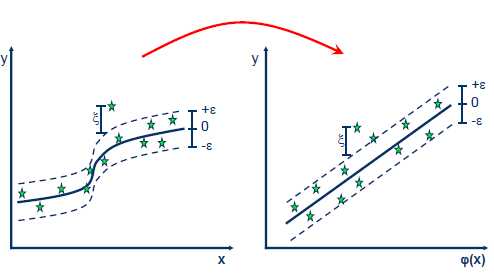
\includegraphics[width=\linewidth]{svr2.png}
 \caption{SVR using kernel}
\end{figure}



\newpage

\subsection{Artificial Neural Networks- Regression}

Neural Network Learning problem: Adjust the connection weights so that the network generates the correct
prediction on the training data.

\begin{figure}[H]
 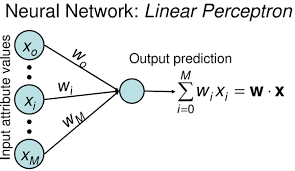
\includegraphics[width=\linewidth]{mneuron.png}
 \caption{Linear Regression Using neural network}
\end{figure}

 The weights Wi can be updated by an algorithm like backpropagation which uses the chain rule to find derivative and calculates how much error each layer adds to the output and updates the weight values accordingly. 


\begin{figure}[H]
 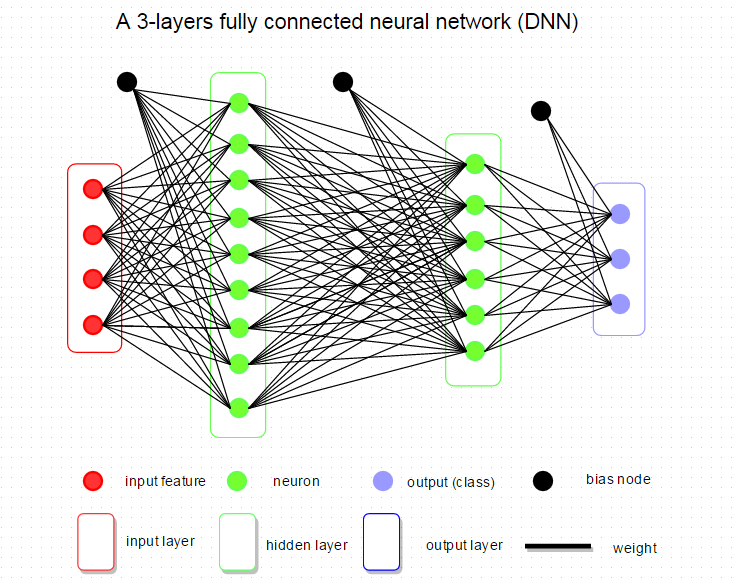
\includegraphics[width=\linewidth]{mneuron1.png}
 \caption{Example of neural network with  2 hidden layers}
\end{figure}


\chapter{Our Work}
The work for our minor project can be broken down into the following steps.\newline
\newline
1. Data gathering\newline\newline
2. Preprocessing\newline\newline
3. Feature extraction\newline\newline
4. Normalization of data\newline\newline
5. Modelling\newline\newline
6. Error calculation
\newpage
\subsection{Data Gathering}
The first two features Closing price and Volume were obtained from google finance historical prices for aapl stocks
and the third feature was obtained using google search engine.\newline\newline
1. Closing price\newline\newline
2. Volume of stocks\newline\newline
3. Google's number of results of that stock for that particular day\newline\newline

And our target variable or output was chosen to be the next day closing price that is close(i+1)
\newpage
\subsection{Preprocessing}
In this step the data obtained is cleaned that is 
\newline\newline
1.Sort the data according to the date
\newline\newline
2.Some of the data from the dataset contains missing values which must be filled for this we resample the data taking samples for each day and interpolate(linear interpolation).
\newline\newline
3.Concatenate the dispartate datasets into one single dataset.
\newpage
\subsection{Feature extraction}
Based on our background study we extract the following features \newline\newline
1. Moving average of the closing price.\newline\newline
		$$Close(n)_{t} = Close_{t}/n + Close_{t-1}/n + ......... + Close_{t-n+1}/n$$
2. Momentum of the closing price\newline
   $$Close(i) + Close(i-1)$$\newline\newline
\newpage
\subsection{Normalization}
Normalization of data is important because of the following reasons-
\newline\newline
1.Normalization of data is important for the model to reach convergence quickly.\newline\newline  
2.Without normalization the data may even never converge to the minimum error.\newline\newline
3.The model might behave badly if the individual features do not more or less look like standard normally distributed data: Gaussian with zero mean and unit variance.\newline\newline
4.In practice we often ignore the shape of the distribution and just transform the data to center it by removing the mean value of each feature, then scale it by dividing non-constant features by their standard deviation.\newline\newline
5.Also  if a feature has a variance that is orders of magnitude larger than others, it might dominate the objective function and make the estimator unable to learn from other features correctly as expected.
\newline\newline
We calculate the mean and standard deviation for the training set and later reapply the same mean and standard deviation in the testing set.
$$Formula for normalization used = X-mean / standard Deviation$$
\newpage
\subsection{Modelling}

We have selected Support Vector regression algorithm to model our data as we had only 30 days of data and SVR works quite well for lower number of training examples and we have used the kernel radial basis function(Rbf). 
\newpage
\subsection{Error calculation}

For this we simply take our predicted data subtract it from the testing set and take the mean.
$$Errors=\sum_{i=1}^{n} (Y(Predicted)[i] - Y[i])/n$$
where n is the number of samples in the testing set.

\chapter{Result and Analysis}
	$$Result = array([ 156.23963679,  162.93297676,  160.45553855,  158.9554201 ,
        161.35103545,  160.52943472])$$
    $$YTestSet = array([ 156.23963679,  162.93297676,  160.45553855,  158.9554201 ,
        161.35103545,  160.52943472])$$
    $$Mean error=\sum_{i=1}^{n} (Y(Predicted)[i] - Y[i])/n$$
    Where n is  number of examples in the testing set    
	$$Mean error = 0.5(approx)$$
	\begin{figure}[H]
 	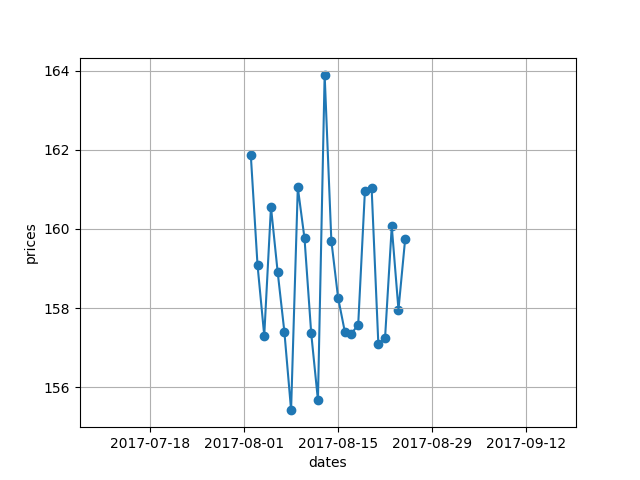
\includegraphics[width=\linewidth]{figure_1-1.png}
 	\caption{Plot of our training data}
	\end{figure}

\chapter{Future Work}
Diversification is possibly the most widely accepted principle in finance. The roots of this concept go as far
back to ancient times where individuals were advised to keep an equal proportion of their wealth in real estate
(land), equities (business), and cash (liquid holdings). However, the modern financial interpretation of
diversification is not well-understood despite its acceptance.
\newline \newline
The idea is to minimize the risk by building a portfolio of stocks to invest upon this can be done by doing correlation
analysis on various stocks and building predictive models on the uncorrelated stocks. After that we can invest on those stocks which are expected to give the highest returns. 

\newpage
\chapter{References}
	1.https://www.quantopian.com \newline \newline
	2.https://www.scikit-learn.org \newline\newline
	3.Application of machine learning techniques for stock market prediction by Bin Weng (A dissertation submitted to the Graduate Faculty of Auburn University in partial fulfillment of the requirements for the Degree of Doctor of PhilosophyAuburn, Alabama May 6, 2017)\newline\newline
	4.The Minimum Correlation Algorithm: A Practical Diversification Tool by Henry Bee, September 2012
\end{document}








